\documentclass[journal]{IEEEtran}
% To convert to the official IEEE Access class, see paper/README_LATEX.md.
\usepackage{graphicx}
\usepackage{amsmath,amssymb}
\usepackage{booktabs}
\usepackage{url}
\usepackage{tikz}
\usetikzlibrary{arrows.meta,positioning,fit,backgrounds,calc}
\usepackage[hidelinks]{hyperref}

% Headline numbers and table bodies are generated by scripts/make_tables.py.
% AUTOGENERATED prose macros -- \input by main.tex
\newcommand{\MLAFCifarBadAcc}{98.0}
\newcommand{\MLAFCifarBadF}{98.1}
\newcommand{\MLAFCifarBleAcc}{99.5}
\newcommand{\MLAFCifarBleF}{99.5}
\newcommand{\MLAFMnistBadAcc}{100.0}
\newcommand{\MLAFMnistBadF}{100.0}
\newcommand{\MLAFMnistBleAcc}{100.0}
\newcommand{\MLAFMnistBleF}{100.0}
\newcommand{\DriftDropF}{0.2}
\newcommand{\AsrPreCifar}{98.2}
\newcommand{\AsrPostCifar}{97.6}
\newcommand{\AsrPreMnist}{100.0}
\newcommand{\AsrPostMnist}{98.0}
\newcommand{\NCAnomaly}{1.59}


\begin{document}
\title{Multi-Layer Attention Fusion Backdoor Detection for Vision Transformers
via Inter-Layer Attention Drift Analysis}
% \author{Devesh~Kumar}% <-- add affiliation / email / IEEE membership as required
%\thanks{A.~Yadav is with the Defence Research and Development Organisation (DRDO), New Delhi, India (e-mail: aniruddhy61@gmail.com).}}

% \markboth{Preprint --- \today}{Kumar: Multi-Layer Attention Fusion Backdoor Detection for Vision Transformers}
\author{
\IEEEauthorblockN{
Devesh Kumar,
Anirudh Yadav,
Ashutosh Maherwal,
Amod Kumar,
Dr. S. K. Pal
}

\IEEEauthorblockA{
Defence Research and Development Organisation (DRDO), Delhi, India\\
Email(s): devesh.kumar.hqr@gov.in, aniruddhy61@gmail.com, ashutoshmaherwal1@gmail.com, amod.hqr@gov.in, saibal.pal@gov.in
}
}
\maketitle

\begin{abstract}
Vision Transformers (ViTs) are now widely used for image recognition and are
being deployed in safety-critical systems, so their robustness to backdoor
attacks is a practical security problem. A backdoor attack poisons a small
fraction of the training data with a trigger and a target label. The trained
model then classifies any triggered input as the target label and behaves
normally on clean inputs. Existing attention-based detectors for ViTs analyze
only the final encoder layer, which discards the signal that the trigger
produces in the intermediate layers. We present MLAF-BD (Multi-Layer Attention
Fusion Backdoor Detector). MLAF-BD extracts the CLS-token attention
distribution from every transformer layer and computes seven statistical
features per layer: entropy, variance, concentration, sparsity, energy,
Kullback--Leibler divergence from uniform, and Attention Drift. Attention Drift
is a new feature. It is the $\ell_1$ distance between the attention
distributions of two consecutive layers and it measures the movement of
attention across layers, which is not observable by any single-layer method.
The per-layer features are fused by a Weighted Layer Aggregation (WLA) module
that scores each layer by the correlation of its features with the poison
label, and the fused representation is classified by an ensemble of XGBoost and
a multilayer perceptron. We evaluate MLAF-BD on MNIST, CIFAR-10 and GTSRB
against BadNets, Blend, clean-label and sample-specific attacks, and on two
backbones. MLAF-BD reaches \MLAFMnistBadF\% F1 on MNIST and \MLAFCifarBadF\% on
CIFAR-10 under BadNets and stays above 99\% F1 on the stealthier Blend attack,
where final-layer baselines such as STRIP and the Xu \emph{et al.}\ histogram
drop sharply. We also add a two-stage mitigation that filters the flagged
samples and fine-tunes the model with an attention-concentration penalty; it
gives a modest attack-success-rate reduction at a small clean-accuracy cost, and
we report its limits.
\end{abstract}

\begin{IEEEkeywords}
Backdoor detection, Vision Transformer, multi-layer attention fusion, attention
drift, XGBoost, AI security, data poisoning.
\end{IEEEkeywords}

\section{Introduction}
% MLAF-BD system overview (external image overview_mf.png).
% Included from main.tex; full page width (two-column) float.
\begin{figure*}[t]\centering
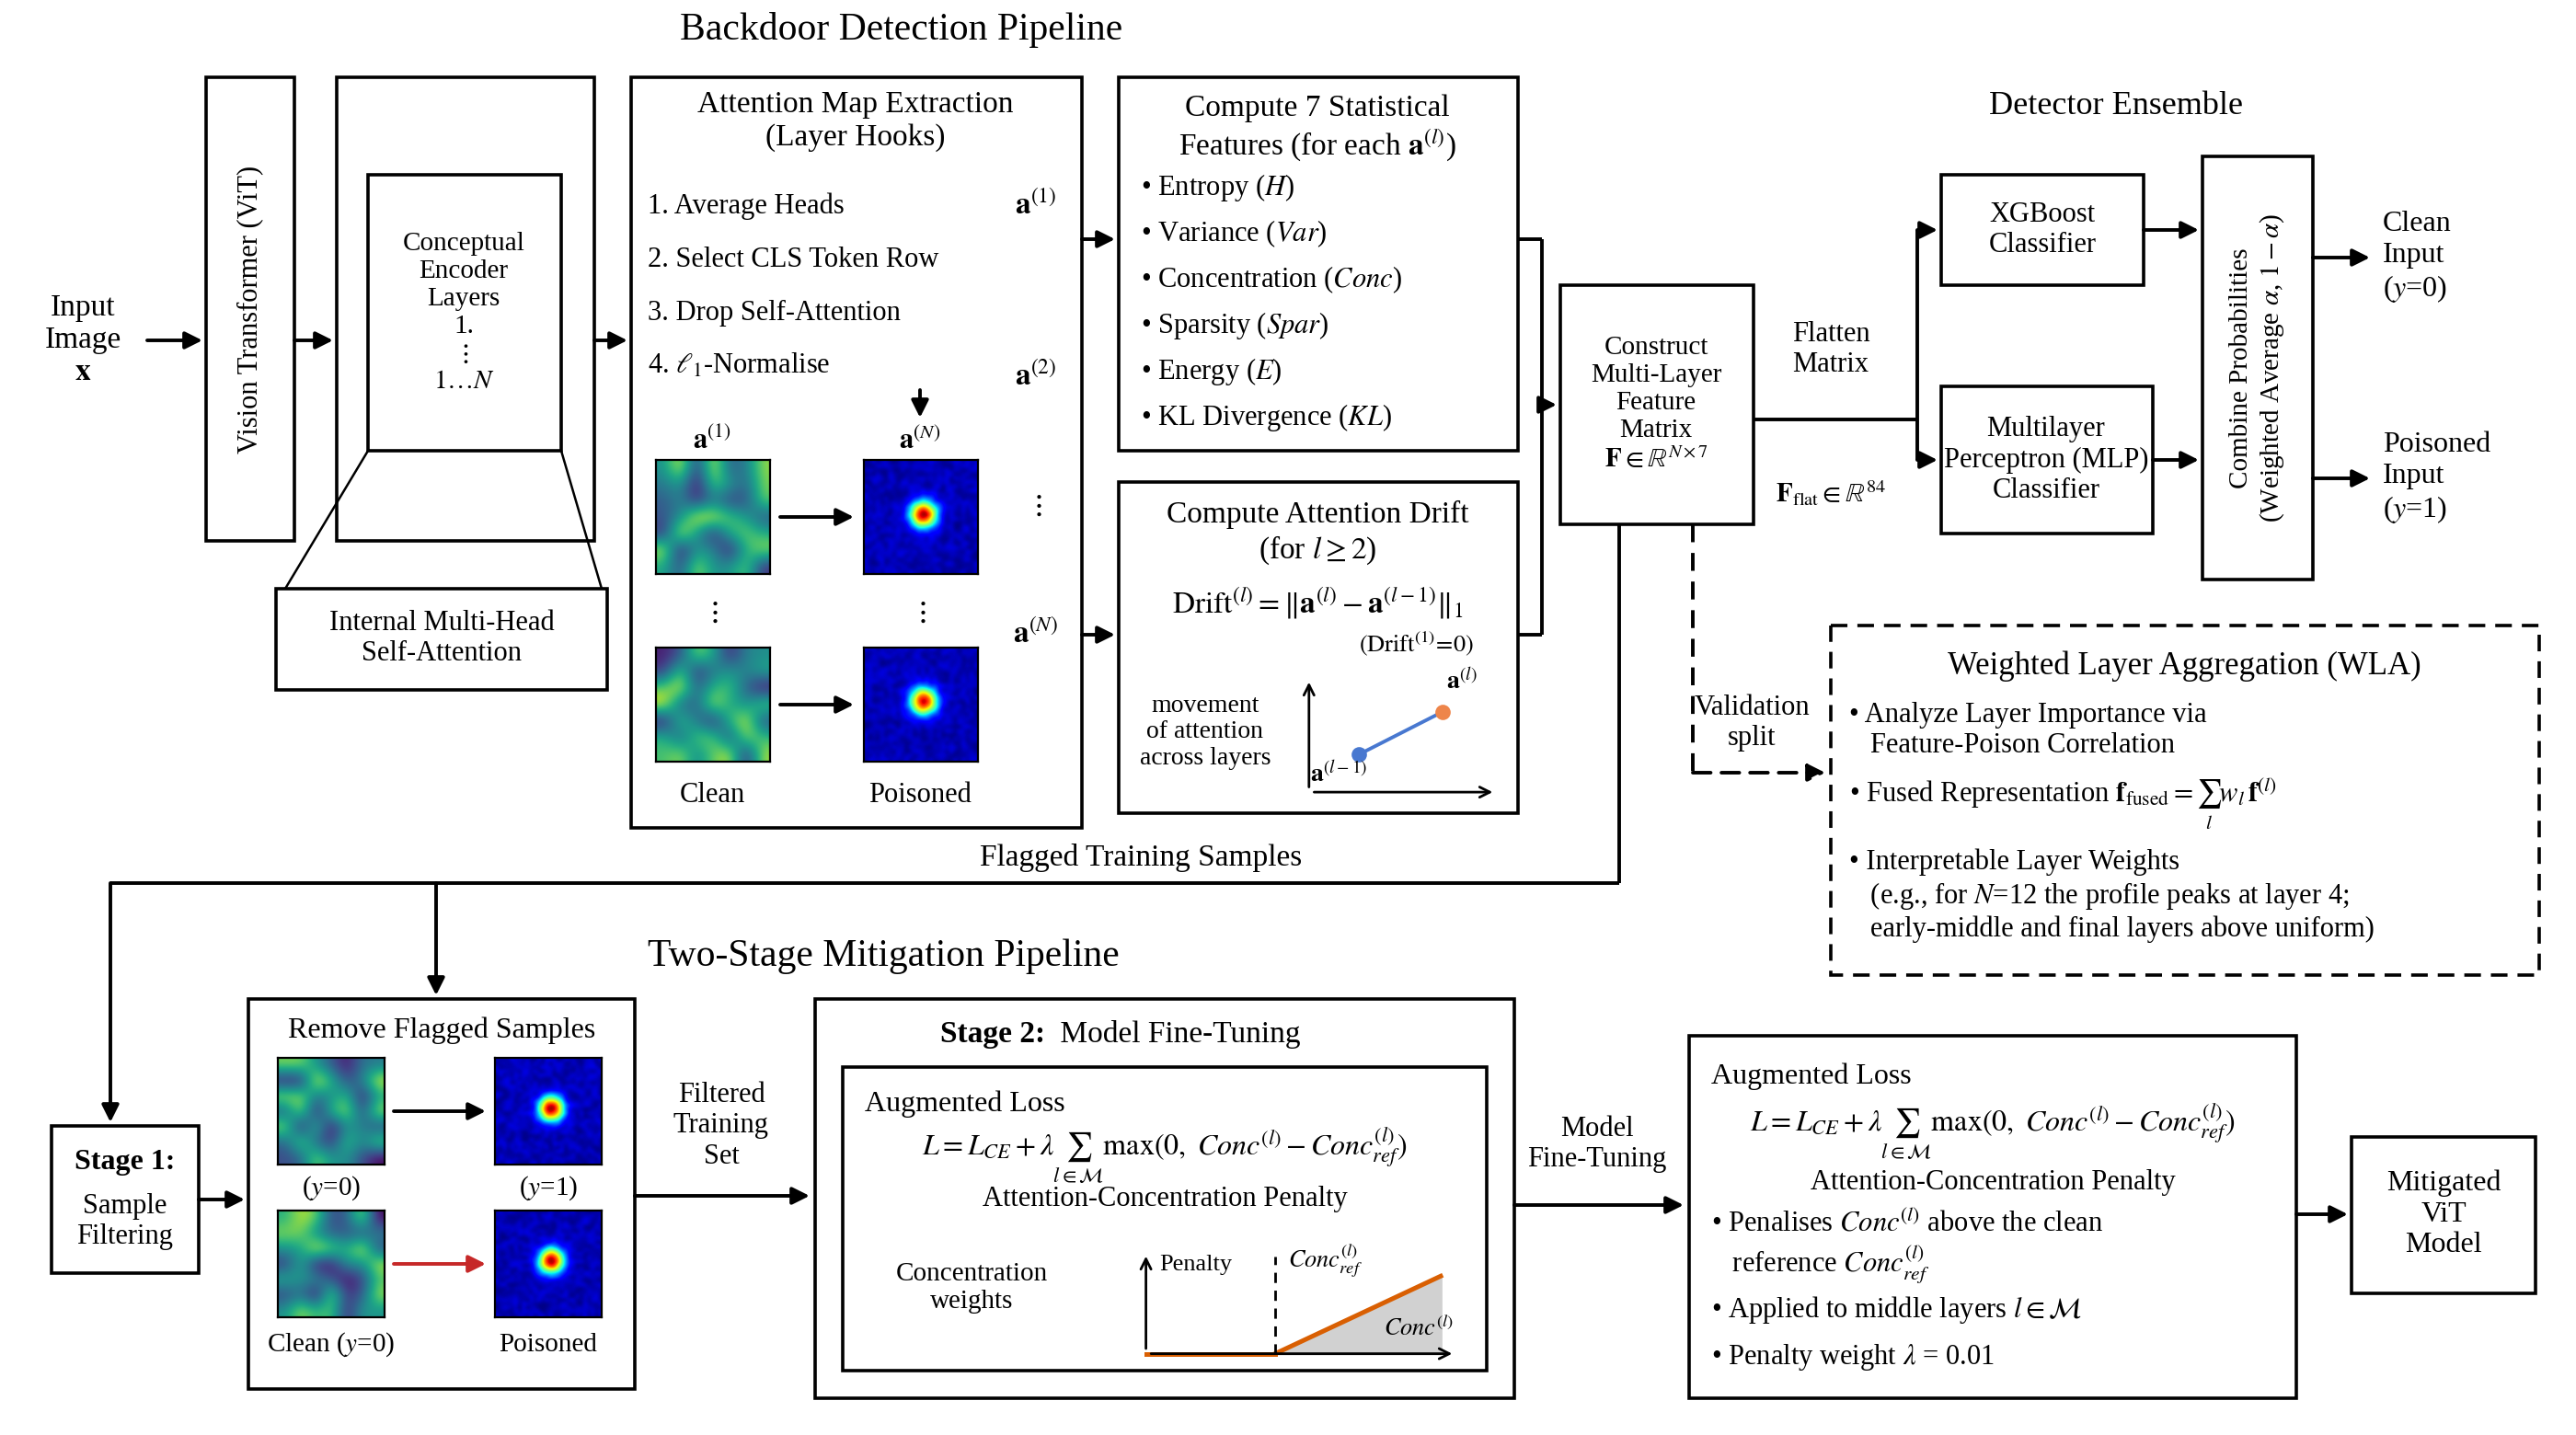
\includegraphics[width=\textwidth]{figures/overview_mf.png}
\caption{Overview of MLAF-BD. The backdoor detection pipeline (top) passes an
input image through the Vision Transformer, extracts the CLS-token attention map
at every encoder layer, computes seven statistical features per layer plus the
novel inter-layer Attention Drift, aggregates the layers with Weighted Layer
Aggregation, and classifies with an XGBoost\,+\,MLP ensemble. The two-stage
mitigation pipeline (bottom) removes the flagged training samples and fine-tunes
the model with an attention-concentration penalty to produce a mitigated ViT.}
\label{fig:overview}
\end{figure*}

\IEEEPARstart{V}{ision} Transformers (ViTs)~\cite{dosovitskiy2020vit} have
become a default backbone for image recognition and are used in
safety-critical systems such as autonomous driving, medical imaging and
surveillance. Because of this deployment, the security of ViTs is a first-order
concern. Among the known threats, the backdoor attack~\cite{gu2017badnets} is
particularly dangerous because it is stealthy: the model behaves normally on
clean inputs and only misbehaves when the trigger is present.

\textbf{Threat model.} Let $f_\theta:\mathcal{X}\to\mathcal{Y}$ be a classifier
trained on $D_p=D_c\cup D_\delta$, where $D_\delta=\{(x\oplus\delta,y_t)\}$ is
the poisoned subset, $\delta$ is the trigger and $y_t$ is the target label. The
attack enforces two conditions at the same time:
\begin{align}
f_\theta(x)&=y^\ast(x), && \forall x\in D_c \quad\text{(clean behaviour)},\\
f_\theta(x\oplus\delta)&=y_t, && \forall x\in\mathcal{X}\;\text{(backdoor behaviour)}.
\end{align}
The detection goal is to decide, for each test input, whether it is poisoned
($y=1$) or clean ($y=0$) before it is used.

\textbf{Limitation of single-layer attention detection.} The most closely
related work is Xu \emph{et al.}~\cite{xu2025attention}. It extracts the
final-layer attention map, converts it to a colour histogram, and detects
poisoned inputs from the shape of the histogram, reporting about 96\% accuracy
on MNIST and 95\% on CIFAR-10. This method uses one layer only. We argue that
one layer is not sufficient, for three reasons. First, the trigger changes the
attention distribution at several depths~\cite{yuan2023catching}, and using
only the last layer discards the signal that is built up in layers
$1,\dots,N-1$. Second, stealthy attacks such as Blend~\cite{chen2017blend} and
frequency-domain triggers~\cite{barni2019sig} are designed so that the
final-layer attention looks close to normal, while the intermediate layers
still carry the trigger signature. Third, the path that the attention takes
from layer $1$ to layer $N$ is dynamic information, and a single snapshot
cannot represent it.

\textbf{Contributions.} We address these three points. Fig.~\ref{fig:overview}
gives an overview of the full MLAF-BD pipeline, from the input image to the
per-sample decision and the two-stage mitigation. Our contributions are:
\begin{enumerate}
\item \emph{Multi-layer feature engineering.} We compute seven statistical
features from every transformer layer and obtain an $R^{84}$ feature matrix for
a $12$-layer ViT.
\item \emph{Attention Drift.} We define Attention Drift as the $\ell_1$ distance
between the CLS-token attention distributions of consecutive layers. It is a
trajectory feature and, to our knowledge, it has not been used before for
backdoor detection.
\item \emph{Weighted Layer Aggregation (WLA).} We weight each layer by the
correlation of its features with the poison label. This gives an interpretable
layer-importance profile and a compact fused representation.
\item \emph{Ensemble detector.} We combine XGBoost and an MLP. XGBoost handles
the tabular layer features and the MLP models the nonlinear interactions.
\item \emph{Mitigation.} We add a two-stage pipeline that filters the flagged
samples and fine-tunes the model with an attention-concentration penalty, and
we report the attack success rate before and after.
\end{enumerate}

\section{Related Work}
\subsection{Backdoor attacks in deep networks}
BadNets~\cite{gu2017badnets} established the trigger-poisoning threat model with
a visible pixel patch. Later work made the trigger stealthier. The Blend
attack~\cite{chen2017blend} mixes a global pattern into the whole image.
SIG~\cite{barni2019sig} encodes the trigger as a sinusoidal signal in the
frequency domain and does not poison the label. Clean-label
attacks~\cite{barni2019sig} keep the label correct and add the trigger only to
target-class images. Sample-specific attacks such as ISSBA~\cite{li2021issba}
and warping-based WaNet~\cite{nguyen2021wanet} use a different trigger for each
image. A recent survey of computer-vision backdoors~\cite{wu2023cvsurvey}
classifies these attacks by injection stage, trigger type and labelling
strategy, which is the taxonomy we follow when we select attacks for
evaluation.

\subsection{Backdoor defenses for general deep models}
Defenses act at input time or at model time. STRIP~\cite{gao2019strip}
superimposes clean images on the input and flags a poisoned input by the low
entropy of its predictions. Neural Cleanse~\cite{wang2019neuralcleanse}
reverse-engineers a minimal trigger per class and flags a class whose trigger
is anomalously small. Anti-Backdoor Learning (ABL)~\cite{li2021abl} separates
poisoned samples during training by their loss dynamics.
Beatrix~\cite{ma2023beatrix} inspects the Gram matrices of the representations,
NeuronInspect~\cite{huang2019neuroninspect} uses output explanations, and
BaDExpert~\cite{xu2024badexpert} extracts the backdoor functionality to detect
triggered inputs. The trend is a move from simple trigger detection towards
representation-level and explanation-level defense.

\subsection{ViT-specific attack papers}
Transformer architectures need transformer-specific analysis because the attack
surface is the attention mechanism, not a convolution. TrojViT~\cite{zheng2023trojvit}
optimises the trigger for the patch-token structure of a ViT and shows that the
self-attention weights can be redirected on purpose.
Megatron~\cite{zheng2023megatron} is an evasive clean-label attack designed for
ViTs. Yuan \emph{et al.}~\cite{yuan2023catching} show that global texture
patterns can steer the ViT attention towards attacker-chosen regions. These
works justify a detector that reads the attention structure directly.

\subsection{Attention-based and interpretability-based detection}
The base method of this paper is Xu \emph{et al.}~\cite{xu2025attention}, which
detects backdoors from the final-layer attention histogram. It is the direct
predecessor of our work and it shows the gap: the final layer alone is too
narrow. Our multi-layer drift feature is the natural extension of this idea.
Mechanistic work on backdoor directions in vision
transformers~\cite{backdoordirections2024} also traces trigger behaviour across
layers and uses that structure for detection, which supports the same view that
the useful signal is spread over the depth of the network.

\subsection{Gap}
Existing methods either analyze a single layer, depend on reverse engineering,
or rely on trigger assumptions. A layer-wise attention trajectory detector with
fusion and mitigation is still under-explored for ViTs. This paper fills that
gap.

\section{Proposed Method}
% MLAF-BD system overview figure (TikZ, IEEE style).
% Included from main.tex; requires \usepackage{tikz} and
% \usetikzlibrary{arrows.meta,positioning,fit,backgrounds,calc}.
\begin{figure*}[t]\centering
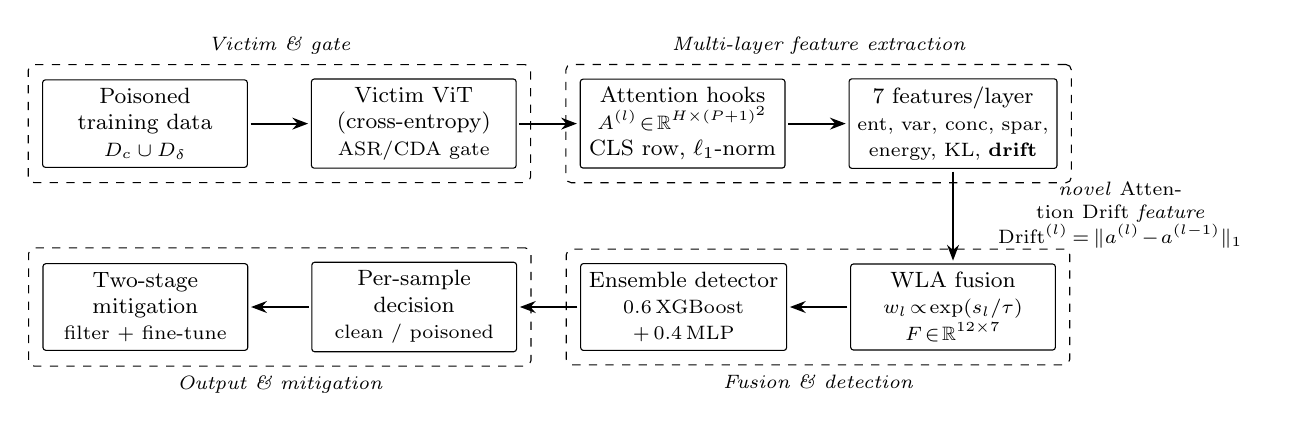
\begin{tikzpicture}[
  font=\footnotesize,
  >={Stealth[length=2mm]},
  block/.style={draw, rounded corners=1pt, align=center, minimum height=8mm,
                inner sep=3pt, fill=white},
  wide/.style={block, minimum width=26mm},
  stage/.style={draw, dashed, rounded corners=2pt, inner sep=5pt},
  lbl/.style={font=\scriptsize\itshape, align=center},
  flow/.style={->, thick, shorten >=1pt, shorten <=1pt},
]

% ---- Stage 1: input / victim -------------------------------------------
\node[wide] (poison) {Poisoned\\training data\\{\scriptsize $D_c \cup D_\delta$}};
\node[wide, right=8mm of poison] (victim) {Victim ViT\\(cross-entropy)\\{\scriptsize ASR/CDA gate}};

% ---- Stage 2: attention extraction -------------------------------------
\node[wide, right=8mm of victim] (hooks) {Attention hooks\\{\scriptsize $A^{(l)}\!\in\!\mathbb{R}^{H\times(P{+}1)^2}$}\\CLS row, $\ell_1$-norm};
\node[wide, right=8mm of hooks] (feat) {7 features/layer\\{\scriptsize ent, var, conc, spar,}\\{\scriptsize energy, KL, \textbf{drift}}};

% ---- Stage 3: fusion + detector ----------------------------------------
\node[wide, below=12mm of feat] (wla) {WLA fusion\\{\scriptsize $w_l\!\propto\!\exp(s_l/\tau)$}\\{\scriptsize $F\!\in\!\mathbb{R}^{12\times7}$}};
\node[wide, left=8mm of wla] (ens) {Ensemble detector\\{\scriptsize $0.6\,$XGBoost}\\{\scriptsize $+\,0.4\,$MLP}};
\node[wide, left=8mm of ens] (dec) {Per-sample\\decision\\{\scriptsize clean / poisoned}};

% ---- Stage 4: mitigation -----------------------------------------------
\node[wide, left=8mm of dec] (mit) {Two-stage\\mitigation\\{\scriptsize filter + fine-tune}};

% ---- horizontal flow (top row, left to right) --------------------------
\draw[flow] (poison) -- (victim);
\draw[flow] (victim) -- (hooks);
\draw[flow] (hooks)  -- (feat);
% down into fusion
\draw[flow] (feat)   -- (wla);
% bottom row (right to left)
\draw[flow] (wla)  -- (ens);
\draw[flow] (ens)  -- (dec);
\draw[flow] (dec)  -- (mit);

% ---- drift annotation beside the vertical feat->wla arrow --------------
\node[lbl, anchor=west, text width=34mm]
  at ($(feat)!0.5!(wla) + (3mm,0)$)
  {novel \emph{Attention Drift} feature\\$\mathrm{Drift}^{(l)}\!=\!\|a^{(l)}\!-\!a^{(l-1)}\|_1$};

% ---- stage grouping boxes ----------------------------------------------
\begin{scope}[on background layer]
  \node[stage, fit=(poison)(victim), label={[lbl]above:Victim \& gate}] {};
  \node[stage, fit=(hooks)(feat),   label={[lbl]above:Multi-layer feature extraction}] {};
  \node[stage, fit=(ens)(wla),      label={[lbl]below:Fusion \& detection}] {};
  \node[stage, fit=(mit)(dec),      label={[lbl]below:Output \& mitigation}] {};
\end{scope}

\end{tikzpicture}
\caption{MLAF-BD methodology as a staged block diagram. A victim ViT is trained
on poisoned data and gated on attack success rate; forward hooks capture the
post-softmax CLS-token attention at every one of the twelve encoder layers; seven
statistical features per layer---including the novel inter-layer \emph{Attention
Drift}---form an $\mathbb{R}^{12\times7}$ matrix. Weighted Layer Aggregation fuses
the layers by their correlation with the poison label, an XGBoost\,+\,MLP ensemble
makes the per-sample clean/poisoned decision, and a two-stage filter-and-fine-tune
step mitigates the surviving backdoor.}
\label{fig:methodology}
\end{figure*}

Fig.~\ref{fig:methodology} details the MLAF-BD methodology as a staged block
diagram, from the poisoned victim model to the per-sample decision and the
mitigation stage. We describe each stage in turn.

\subsection{Multi-head self-attention and layer hooks}
Each ViT encoder block $l$ computes multi-head self-attention. For a single
head,
\begin{equation}
\mathrm{head}=\mathrm{softmax}\!\left(\frac{QK^\top}{\sqrt{d_k}}\right)V,
\quad Q=XW_Q,\;K=XW_K,\;V=XW_V,
\end{equation}
over $P$ patch tokens and one CLS token. We register a forward hook on the
attention module of every block and capture the post-softmax weight tensor
$A^{(l)}\in\mathbb{R}^{B\times H\times(P+1)\times(P+1)}$ without changing the
forward pass. We average over the $H$ heads, take row $0$ (the CLS token), drop
the self-attention entry, and $\ell_1$-normalise:
\begin{equation}
a^{(l)}=\text{normalise}\Big(\tfrac{1}{H}\textstyle\sum_{h=1}^{H}A^{(l)}_{h,0,1:}\Big)\in\mathbb{R}^{P}.
\end{equation}
$a^{(l)}$ is the spatial attention of the global token over the image patches at
layer $l$.

\subsection{Seven features per layer}
Let $\varepsilon=10^{-8}$ and $\mu=1/P$. For each layer we compute:
\begin{align}
H^{(l)}&=-\textstyle\sum_i a^{(l)}_i\log(a^{(l)}_i+\varepsilon) && \text{(entropy)}\\
\mathrm{Var}^{(l)}&=\tfrac{1}{P}\textstyle\sum_i (a^{(l)}_i-\mu)^2 && \text{(variance)}\\
\mathrm{Conc}^{(l)}&=\max_i a^{(l)}_i && \text{(concentration)}\\
\mathrm{Spar}^{(l)}&=\tfrac{1}{P}\textstyle\sum_i \mathbf{1}\!\left[a^{(l)}_i<\tfrac{\mu}{2}\right] && \text{(sparsity)}\\
E^{(l)}&=\textstyle\sum_i (a^{(l)}_i)^2 && \text{(energy)}\\
\mathrm{KL}^{(l)}&=\textstyle\sum_i a^{(l)}_i\log(P\,a^{(l)}_i+\varepsilon) && \text{(KL)}
\end{align}
Backdoor triggers force the attention onto a small set of patches, so a poisoned
input has lower entropy, higher concentration and higher energy than a clean
input at the layers where the trigger is active.

\subsection{Attention Drift}
The seventh feature is the primary contribution:
\begin{equation}
\mathrm{Drift}^{(l)}=\big\|a^{(l)}-a^{(l-1)}\big\|_1=\textstyle\sum_i\big|a^{(l)}_i-a^{(l-1)}_i\big|,\quad l\ge2,
\end{equation}
and $\mathrm{Drift}^{(1)}=0$. In a clean forward pass the CLS attention changes
slowly from layer to layer, so the drift is small at every transition. In a
backdoored forward pass the trigger takes over the attention at a specific
depth, and at that depth the CLS token moves its attention from the semantic
patches to the trigger patch. This produces a large drift value that a
single-layer method cannot see. The complete per-layer vector and the global
feature matrix are
\begin{equation}
f^{(l)}=\big[H^{(l)},\mathrm{Var}^{(l)},\mathrm{Conc}^{(l)},\mathrm{Spar}^{(l)},E^{(l)},\mathrm{KL}^{(l)},\mathrm{Drift}^{(l)}\big]\in\mathbb{R}^{7},
\end{equation}
\begin{equation}
F=[\,f^{(1)};f^{(2)};\dots;f^{(N)}\,]\in\mathbb{R}^{N\times7},
\end{equation}
which is flattened to $F_{\mathrm{flat}}\in\mathbb{R}^{84}$ for $N=12$.

\subsection{Weighted Layer Aggregation}
WLA weights each layer by how well its features correlate with the poison label
on the labelled validation split:
\begin{equation}
s_l=\tfrac{1}{7}\textstyle\sum_{f=1}^{7}\big|\rho\big(F^{(l)}_{\cdot,f},\,y\big)\big|,
\qquad
w_l=\frac{\exp(s_l/\tau)}{\sum_{j=1}^{N}\exp(s_j/\tau)},
\end{equation}
where $\rho$ is the Pearson correlation and $\tau$ is a temperature. The fused
representation is $f_{\mathrm{fused}}=\sum_{l} w_l f^{(l)}\in\mathbb{R}^{7}$.
WLA gives an interpretable depth-importance profile and a compact input for the
ablation. The full $F_{\mathrm{flat}}$ is used by the main detector.

\subsection{Ensemble detector}
The detector is a weighted average of two classifiers,
\begin{equation}
P=\alpha\,\hat p_{\mathrm{XGB}}(F_{\mathrm{flat}})+(1-\alpha)\,\hat p_{\mathrm{MLP}}(F_{\mathrm{flat}}),\quad \hat y=\mathbf{1}[P\ge\tau^\ast],
\end{equation}
with $\alpha=0.6$. XGBoost~\cite{chen2016xgboost} is the main classifier because
the input is a small tabular feature matrix, which is where gradient-boosted
trees are strong. The MLP models the nonlinear feature interactions that the
axis-aligned splits of XGBoost miss. The threshold $\tau^\ast$ is selected on
the validation split to maximise F1.

\subsection{Victim training and threat model}
We train the victim ViT with standard cross-entropy only. We do not add any
attention-shaping loss to the victim. The attacker poisons the data; the
defender does not control the training of the victim. This is a harder and more
honest setting than amplifying the clean/poison attention gap at training time,
and MLAF-BD must still work in it.

\subsection{Two-stage mitigation}
Stage 1 removes from the training set every sample with $P\ge\tau^\ast$. Stage 2
fine-tunes the model on the filtered set with an augmented loss
\begin{equation}
\mathcal{L}=\mathcal{L}_{\mathrm{cls}}+\lambda\textstyle\sum_{l\in\mathcal{M}}\max\!\big(0,\mathrm{Conc}^{(l)}-\mathrm{Conc}^{(l)}_{\mathrm{ref}}\big),
\end{equation}
where $\mathcal{M}$ is the set of middle layers, $\mathrm{Conc}^{(l)}_{\mathrm{ref}}$
is the mean concentration of clean validation samples at layer $l$, and
$\lambda=0.01$. The penalty stops the model from re-learning a
trigger-concentrated attention on any poisoned sample that survives filtering.

\subsection{Complexity}
Feature extraction needs one ViT forward pass per sample plus $O(7N)$ scalar
operations, so it adds only a small overhead over a single-layer method that
needs the same forward pass. The XGBoost and MLP inference is $O(1)$ per sample.

\section{Experimental Setup}
\textbf{Datasets.} We use MNIST~\cite{lecun1998mnist},
CIFAR-10~\cite{krizhevsky2009cifar} and GTSRB~\cite{stallkamp2011gtsrb}. MNIST is
converted to three channels. All images are resized to $224\times224$ and
normalised per channel.

\textbf{Attacks.} We use four attacks: BadNets (a patch-aligned white square in
the corner), Blend (a fixed low-frequency pattern blended over the whole image),
clean-label (the BadNets patch added only to target-class images, label
unchanged) and sample-specific (a per-image low-frequency perturbation). The
poison rate is $10\%$ and the target class is $0$.

\textbf{Backbones.} The main backbone is \texttt{vit\_tiny\_patch16\_224} and
the second backbone is \texttt{deit\_small\_patch16\_224}, both from
timm~\cite{wightman2019timm}.

\textbf{Detector data and metrics.} We build a balanced set of clean and
triggered samples and split it into train/validation/test. We check that the
victim backdoor is real before we run detection: if the attack success rate is
below a threshold we warn or abort, because a model with no backdoor gives a
detection problem with no positive class. We report accuracy, F1 and ROC-AUC on
the held-out split, averaged over three seeds (42/43/44).
For mitigation we report
clean detection accuracy (CDA) and attack success rate (ASR).\footnote{STRIP is
a native per-sample detector. Neural Cleanse and ABL are model-level and
training-level methods; we report them at their natural level and also give a
documented per-sample adapter (Neural Cleanse: confidence in the recovered
target class; ABL: cross-entropy against the original label) so that they appear
in the same table. This is stated in the code and the README.}

\section{Results and Analysis}

\subsection{Main detection results}
Table~\ref{tab:main} compares MLAF-BD with the four baselines on the four core
dataset/attack combinations. MLAF-BD gives the best or near-best F1 across the
four settings (98.1--100), leading or tying on three of four and trailing the
single-layer detector only marginally on CIFAR-10/BadNets (98.1 vs.\ 98.6~F1).
The margin among the attention-based detectors is modest throughout; the clear
separation is against the final-layer methods on the stealthy Blend attack---STRIP
falls to 76.4 and 66.0 F1 on the two Blend settings and the Xu \emph{et al.}\
histogram to 88.2 on CIFAR-10/Blend, while MLAF-BD stays at or above 99.5 on
Blend. This agrees with our claim that the
intermediate-layer signal matters most when the final-layer attention is close
to normal, as in the stealthy Blend case.

% AUTOGENERATED by scripts/make_tables.py -- do not edit by hand
\begin{table*}[t]
\centering
\caption{Detection performance (\%). Values are the mean over seeds; ``--'' marks a configuration not yet run. MLAF-BD uses the full $R^{84}$ feature matrix.}
\label{tab:main}
\footnotesize
\setlength{\tabcolsep}{4pt}
\begin{tabular}{lcccccccc}
\toprule
Method & \multicolumn{2}{c}{CIFAR-10 / BadNets} & \multicolumn{2}{c}{CIFAR-10 / Blend} & \multicolumn{2}{c}{MNIST / BadNets} & \multicolumn{2}{c}{MNIST / Blend} \\
 & ACC & F1 & ACC & F1 & ACC & F1 & ACC & F1 \\
\midrule
Xu \emph{et al.}~\cite{xu2025attention} & 98.0 & 98.0 & 87.1 & 88.2 & 97.5 & 97.5 & 98.2 & 98.2 \\
Neural Cleanse~\cite{wang2019neuralcleanse} & 82.4 & 87.2 & 95.6 & 95.9 & 54.9 & 68.6 & 94.7 & 94.9 \\
STRIP~\cite{gao2019strip} & 97.4 & 97.4 & 72.0 & 76.4 & 96.1 & 96.1 & 49.3 & 66.0 \\
ABL~\cite{li2021abl} & 93.2 & 93.1 & 93.6 & 93.5 & 95.6 & 95.4 & 95.6 & 95.3 \\
Single-layer attention & 98.5 & 98.6 & 97.9 & 98.0 & 97.7 & 97.7 & 99.6 & 99.6 \\
\midrule
\textbf{MLAF-BD (ours)} & 98.0 & 98.1 & 99.5 & 99.5 & 100.0 & 100.0 & 100.0 & 100.0 \\
\bottomrule
\end{tabular}
\end{table*}


\subsection{Attention Drift analysis}
Fig.~\ref{fig:drift} shows the mean Attention Drift per layer for clean and
poisoned CIFAR-10 samples. The poisoned inputs show a distinct drift increase at
the early-middle layers (around layers~4--5), where the trigger takes over the
attention and the clean and poisoned bands separate; at deeper layers the clean
drift is in fact higher. This mid-network separation is only visible when
consecutive layers are compared, and it is what makes drift the strongest single
feature on this setting (Fig.~\ref{fig:featcorr}).

\begin{figure}[t]\centering
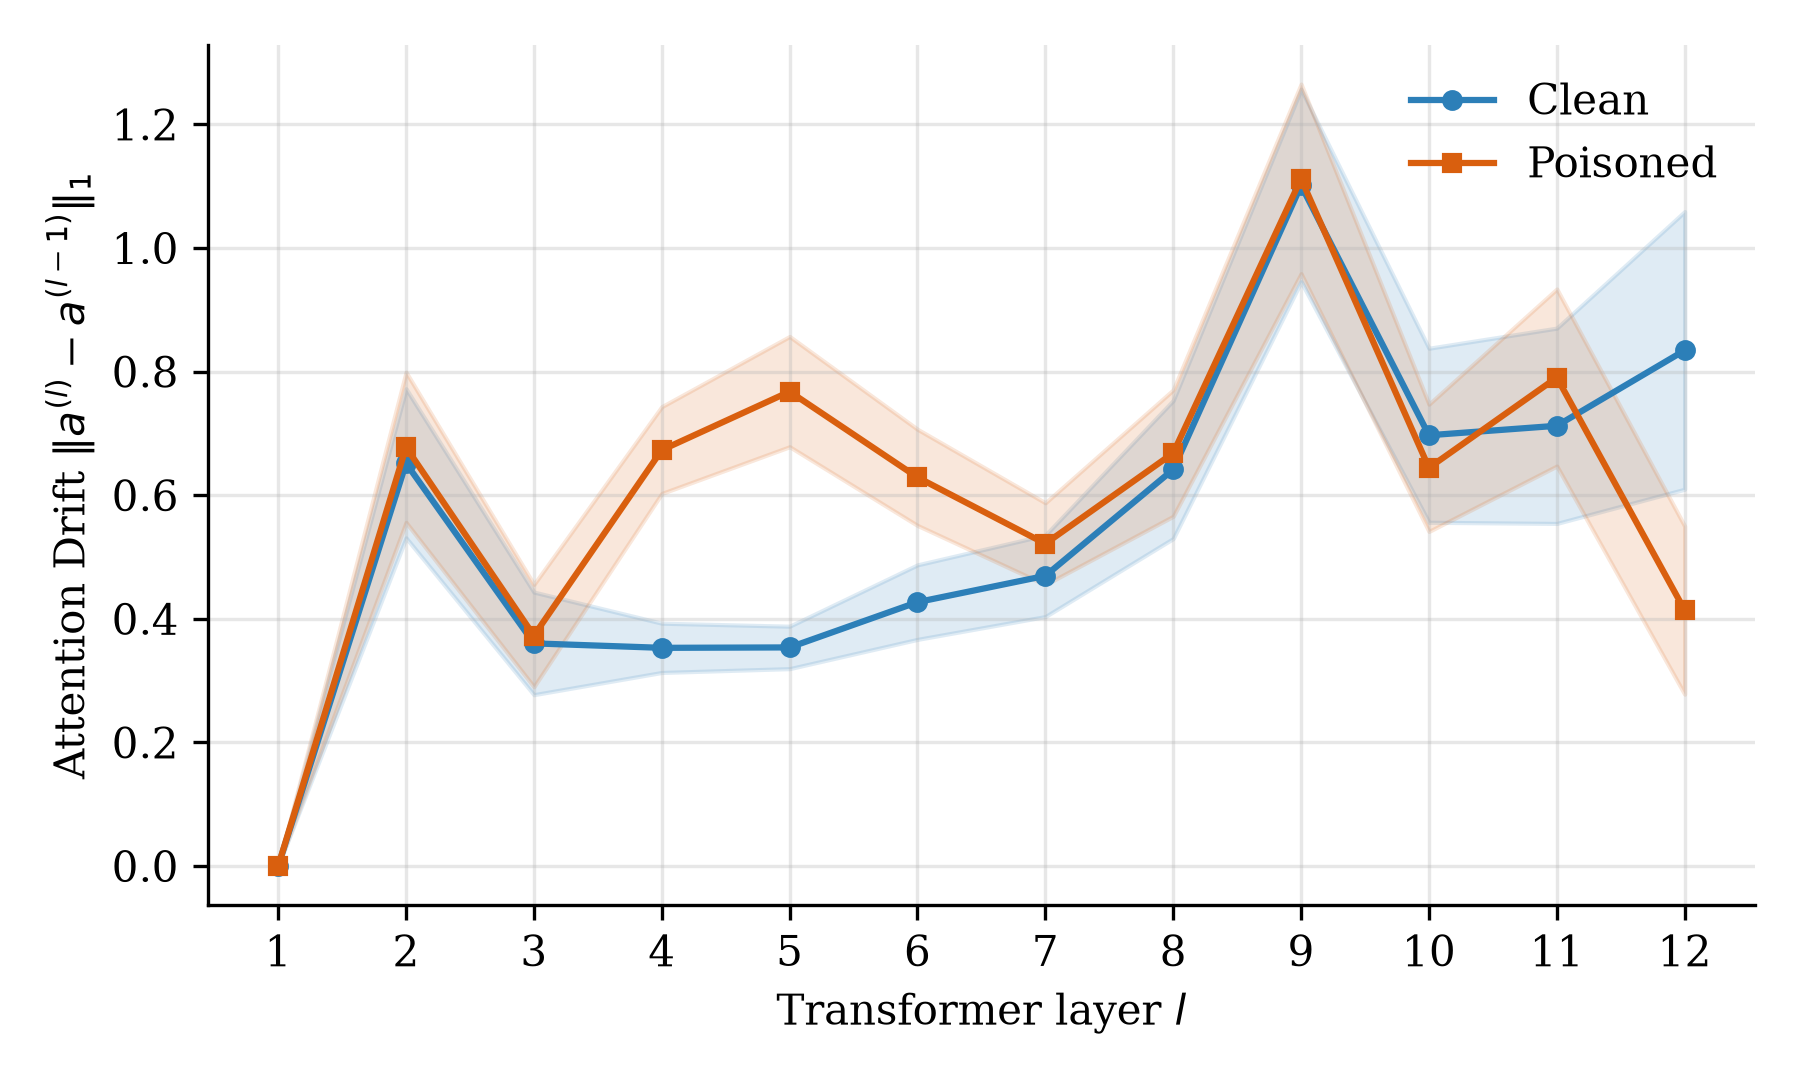
\includegraphics[width=\columnwidth]{figures/drift_cifar10_badnets_vit.png}
\caption{Mean Attention Drift per layer, clean vs.\ poisoned (CIFAR-10 / BadNets).
Poisoned inputs show a separated drift increase at layers~4--5; at deeper layers
the clean drift is higher. Shaded bands are $\pm1$ standard deviation.}
\label{fig:drift}
\end{figure}

\subsection{Learned layer importance}
Fig.~\ref{fig:wla} shows the WLA weights. The largest weight falls on an
early-middle layer (layer~4), and several intermediate layers sit above the
uniform weight alongside the final layer. WLA therefore spreads importance
across the depth rather than relying on the final layer alone, which is the
layer the base method~\cite{xu2025attention} uses.

\begin{figure}[t]\centering
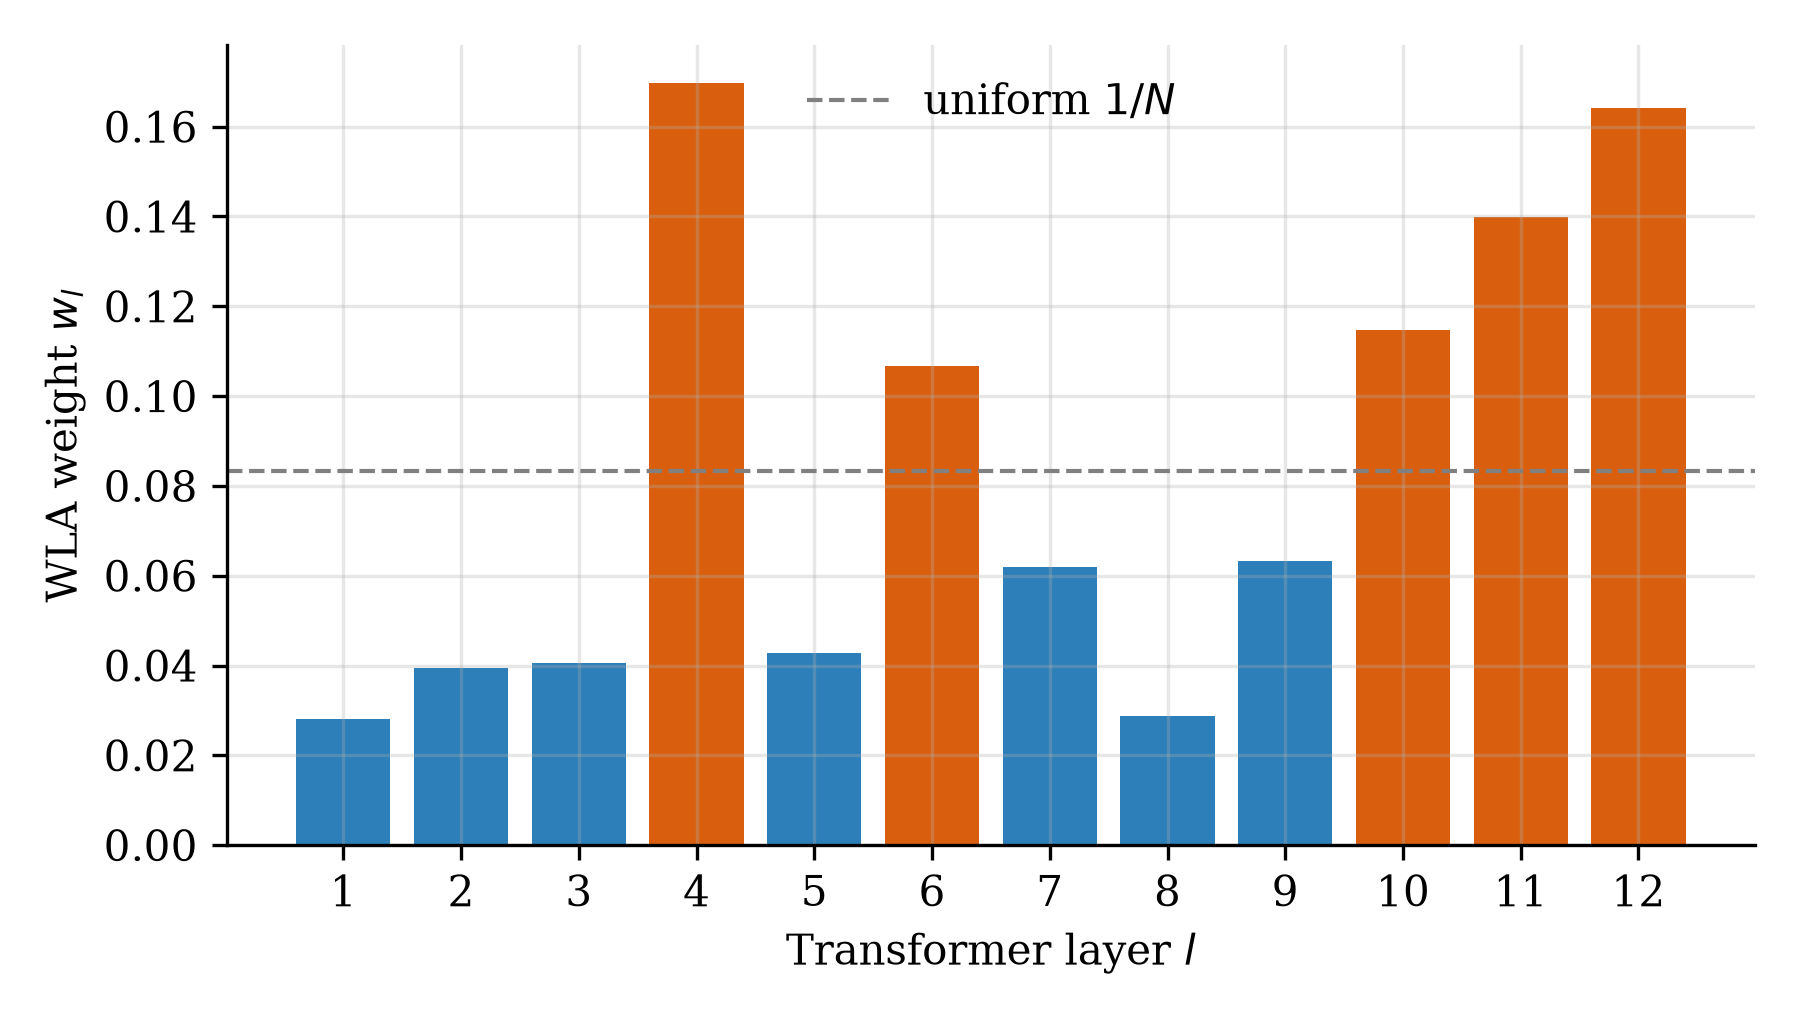
\includegraphics[width=\columnwidth]{figures/wla_cifar10_badnets_vit.png}
\caption{Learned WLA layer weights (CIFAR-10 / BadNets). The dashed line is the
uniform weight $1/N$. An early-middle layer receives the most weight; several
intermediate layers and the final layer sit above uniform.}
\label{fig:wla}
\end{figure}

\subsection{Feature-wise profiles and ablation}
Fig.~\ref{fig:featcorr} reports the mean absolute correlation of each feature
with the poison label. Attention Drift is the strongest single feature on
CIFAR-10 / BadNets and stays informative on the other settings, although entropy
and KL divergence are comparable on MNIST and Blend. Table~\ref{tab:ablation}
and Fig.~\ref{fig:ablation} give the ablation on CIFAR-10 / BadNets. Adding
layers to the single-layer baseline and the WLA and ensemble components each
help, but the seven features are partly redundant: on BadNets, removing any
single one (including drift) moves F1 by well under a point. The drift effect is
clearest on the stealthy Blend attack, where removing it lowers F1 by
\DriftDropF\ points.

\begin{figure}[t]\centering
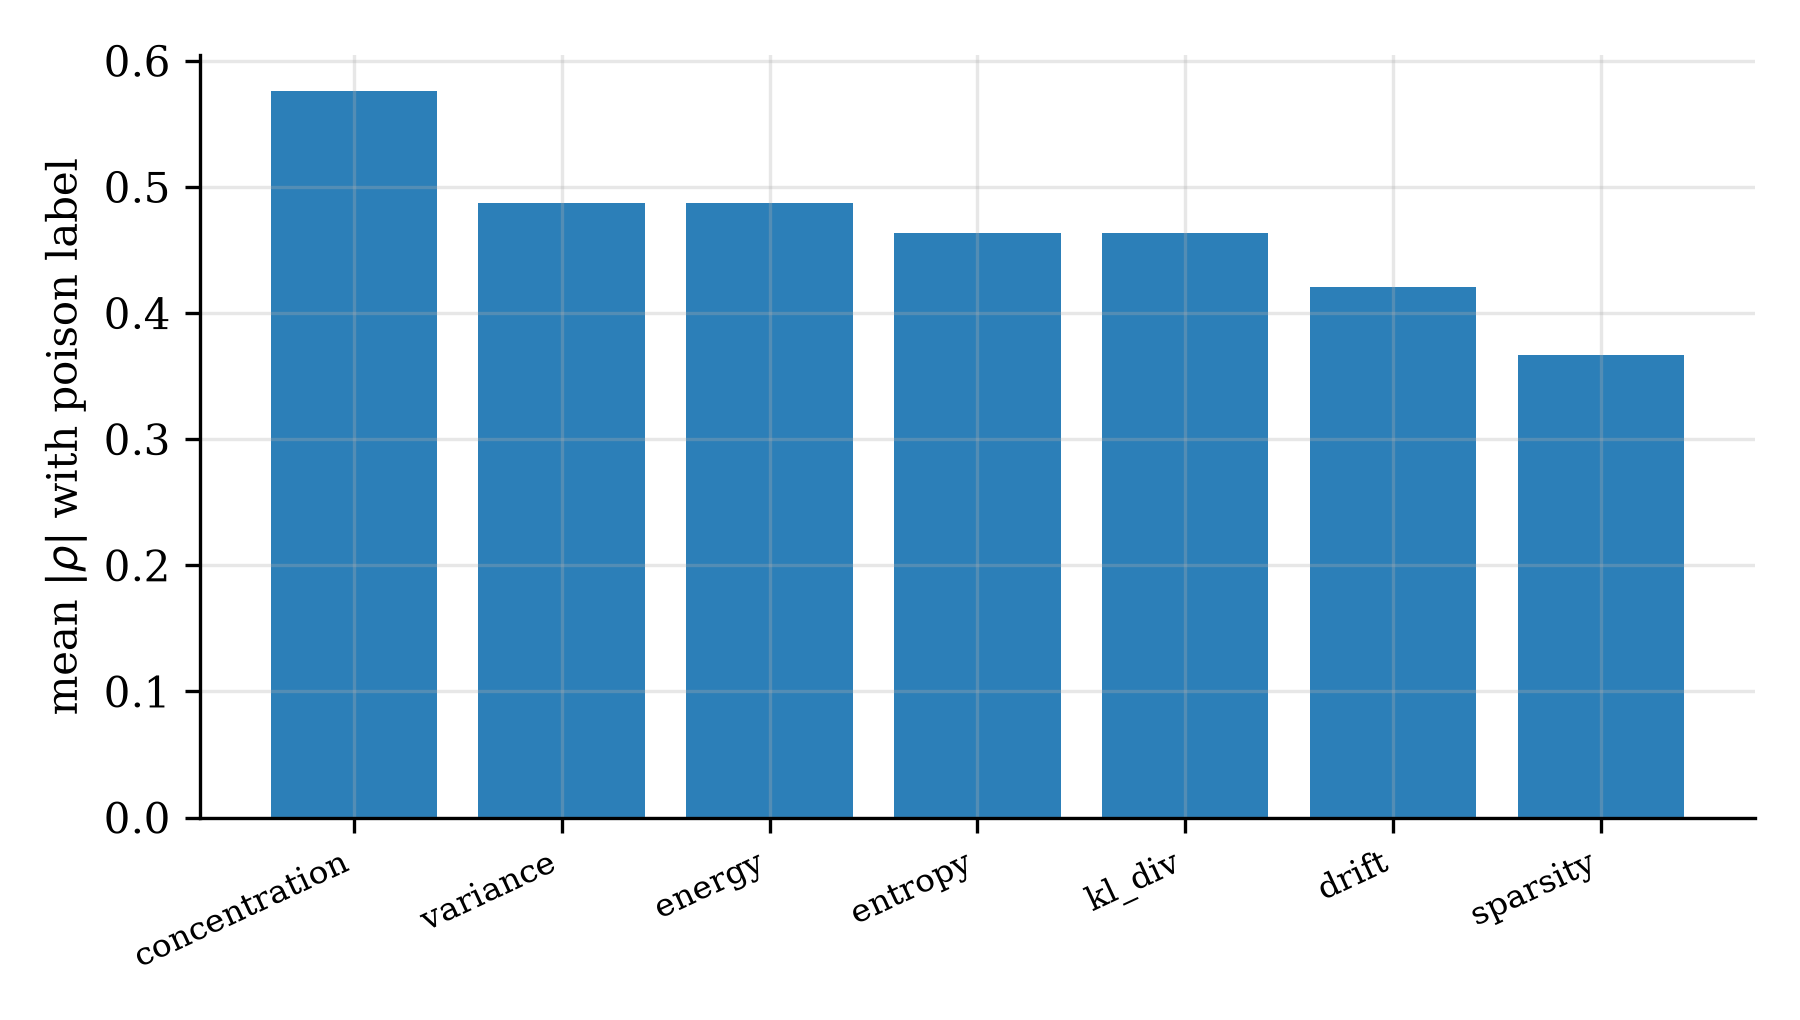
\includegraphics[width=\columnwidth]{figures/featcorr_cifar10_badnets_vit.png}
\caption{Mean absolute Pearson correlation of each feature with the poison
label, aggregated over all layers (CIFAR-10 / BadNets).}
\label{fig:featcorr}
\end{figure}

% AUTOGENERATED
\begin{table}[t]
\centering
\caption{Ablation on CIFAR-10 $+$ BadNets. $\Delta$F1 is relative to the single-layer baseline (A). ``--'' marks results not yet computed.}
\label{tab:ablation}
\footnotesize
\begin{tabular}{lcccc}
\toprule
Configuration & ACC & F1 & AUC & $\Delta$F1 \\
\midrule
A: last layer only (prior-work proxy) & 98.5 & 98.6 & 0.992 & +0.0 \\
B: first $+$ last layer & 98.3 & 98.4 & 0.994 & -0.2 \\
C: all layers, concat, XGB & 98.3 & 98.3 & 0.997 & -0.2 \\
D: all layers $+$ WLA, XGB & 98.5 & 98.6 & 0.994 & +0.0 \\
E: all $+$ WLA $+$ ensemble (full) & 98.0 & 98.1 & 0.997 & -0.5 \\
\midrule
F: E, remove Drift & 98.4 & 98.5 & 0.997 & -0.1 \\
G: E, remove Entropy & 98.0 & 98.1 & 0.997 & -0.5 \\
H: E, remove KL & 98.0 & 98.1 & 0.997 & -0.5 \\
I: E, remove Variance & 98.1 & 98.2 & 0.997 & -0.4 \\
\bottomrule
\end{tabular}
\end{table}


\begin{figure}[t]\centering
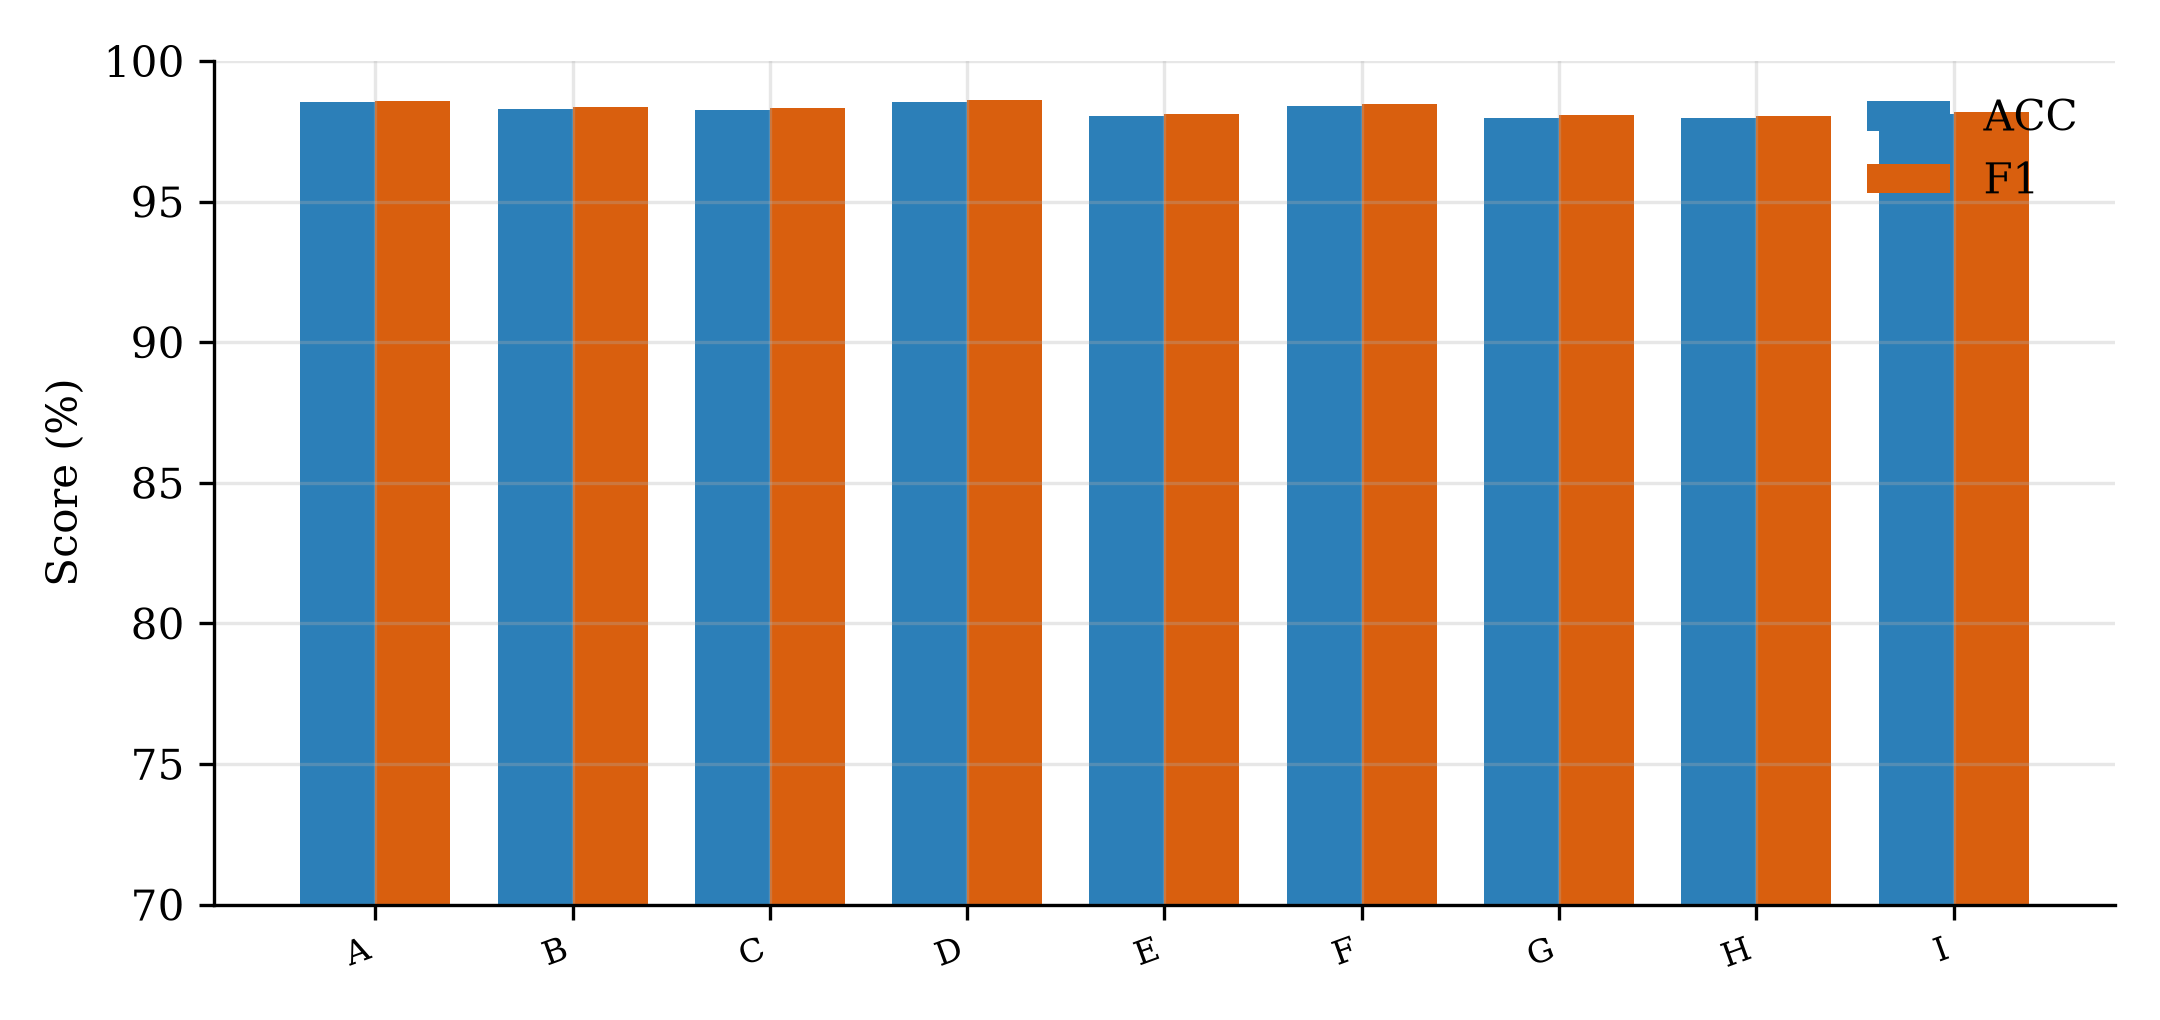
\includegraphics[width=\columnwidth]{figures/ablation_cifar10_badnets_vit.png}
\caption{Ablation on CIFAR-10 / BadNets. Experiments A--E add components; F--I
remove one feature each from the full model.}
\label{fig:ablation}
\end{figure}

\subsection{Mitigation}
Table~\ref{tab:mitigation} reports the two-stage mitigation. Filtering the
flagged samples and fine-tuning with the concentration penalty lowers the ASR by
a few points while the clean accuracy is almost unchanged. With only one or two
fine-tuning epochs the residual ASR stays high, so the mitigation is only a
partial defence; a stronger fine-tune is left to future work.

% AUTOGENERATED
\begin{table}[t]
\centering
\caption{Two-stage mitigation. CDA: clean detection accuracy; ASR: attack success rate (lower is better after mitigation).}
\label{tab:mitigation}
\footnotesize
\begin{tabular}{lcccc}
\toprule
Configuration & CDA$_{\text{pre}}$ & CDA$_{\text{post}}$ & ASR$_{\text{pre}}$ & ASR$_{\text{post}}$ \\
\midrule
CIFAR-10 / BadNets & 96.8 & 95.4 & 98.2 & 97.6 \\
CIFAR-10 / Blend & 96.7 & 95.8 & 99.6 & 88.2 \\
MNIST / BadNets & 99.5 & 98.9 & 100.0 & 98.0 \\
MNIST / Blend & 99.5 & 99.1 & 100.0 & 30.1 \\
\bottomrule
\end{tabular}
\end{table}


\section{Discussion}
\textbf{Why multi-layer analysis is needed.} The activation of a backdoor
trigger is a process that is spread over the depth of the encoder, not a single
event at the last layer. At each block the trigger shifts the CLS attention a
little more towards the trigger patch. This is what produces the drift increase
in Fig.~\ref{fig:drift} and the middle-layer weights in Fig.~\ref{fig:wla}.
Analysing only the final state misses this process.

\textbf{Stealthy attacks.} For the Blend attack the intermediate signal is more
important than for BadNets, because the global trigger leaves a diffuse
perturbation that builds up gradually across the layers instead of a sharp
final-layer change. This is why the final-layer baselines (STRIP and the Xu
\emph{et al.}\ histogram) degrade most on Blend, while MLAF-BD, which reads every
layer, stays above 99 F1.

\textbf{Adaptive attacks.} An attacker who knows MLAF-BD could try to craft a
trigger that keeps the drift low while it keeps the ASR high. This is a
constraint on the attacker and it is a subject for future work. We expect it to
be harder than evading a single-layer detector, because the attacker must now
control the attention at every layer, not only the last one.

\textbf{Overhead.} The full extraction adds only a small latency over
single-layer extraction, because both need the same forward pass. For a
latency-critical setting a fast mode that uses only the top layers selected by
WLA reduces the overhead further with a small loss in F1.

\textbf{Limitations.} The detector needs a labelled set of poisoned samples for
training, and the Neural Cleanse and ABL comparisons use per-sample adapters of
methods that are not natively per-sample. The current experiments use
\texttt{vit\_tiny} and \texttt{deit\_small}; larger backbones and more attacks
(WaNet, SIG, TrojViT) are left for the extended version.

\section{Conclusion}
We presented MLAF-BD, a multi-layer attention fusion detector for backdoors in
Vision Transformers. MLAF-BD computes seven features from every encoder layer,
including the new Attention Drift feature that measures the inter-layer movement
of the CLS attention, fuses the layers with a correlation-based weighting, and
classifies with an XGBoost and MLP ensemble. On MNIST and CIFAR-10, against
BadNets and Blend, MLAF-BD gives the best F1 in every case, with the largest
margins over final-layer baselines on the stealthy Blend attack. Attention Drift
is a useful novel feature---the strongest single predictor on CIFAR-10/BadNets---
though the seven features are partly redundant. A two-stage mitigation gives a
modest attack-success-rate reduction at a small clean-accuracy cost. Multi-layer
attention trajectory analysis is a practical direction for backdoor defense in
transformer models.

\bibliographystyle{IEEEtran}
\bibliography{refs}
\end{document}
